%-------------------------------------------------------------------------------
% File: user_manual_CH2.tex
%       Part of StockSim project documentation.
%       See main.tex for further information.
%-------------------------------------------------------------------------------
\chapter{StockSim Client Manual}
The StockSim Client has two different running modes: the first one
\begin{lstlisting}[basicstyle=\footnotesize\ttfamily,language=bash,numbers=left,
numberstyle=\footnotesize,numbersep=8pt,frame=single]
Welcome to the StockSim Client.

*** [RUNNING IN USER MODE] ***

Available Commands:
register         create a new user account.              
login            login to your user account.             
quit             quit StockSim client. 
\end{lstlisting}
is the \texttt{user mode}. Whereas, the second running mode can be triggered 
using the \texttt{--admin} command line argument:
\begin{lstlisting}[basicstyle=\footnotesize\ttfamily,language={},numbers=left,
numberstyle=\footnotesize,numbersep=8pt,frame=single]
$ java -jar Client.jar --admin

Welcome to the StockSim Client.

*** [RUNNING IN ADMIN MODE] ***

Available Commands:
login        login to your admin account.            
quit         quit StockSim client.
\end{lstlisting}
and is the \texttt{admin mode}. Although they might look like the same, the 
available menu actions differ once the user/admin login has been executed.

\section{StockSim Client User Mode}
Upon launching the application in \textit{user} mode, the user is presented with three options: \textit{register}, \textit{login} and \textit{quit}.\\
After selecting \textit{register}, the user is asked to enter their info, such as name, surname, email, username and password:
\begin{lstlisting}[basicstyle=\footnotesize\ttfamily,language={},numbers=left,
numberstyle=\footnotesize,numbersep=8pt,frame=single]
> register
Name: John
Surname: Smith
E-Mail: jsmith@example.com
Username [login]: jsmith
Password [login]: hunter2
User sign up executed correctly. You can now login.
\end{lstlisting}

Once the user is registered and logged in, the application offers several options:

\begin{lstlisting}[basicstyle=\footnotesize\ttfamily,language={},numbers=left,
numberstyle=\footnotesize,numbersep=8pt,frame=single]
> login
Username: jsmith
Password: hunter2
User login executed correctly.
Welcome John Smith.

[jsmith] Available Commands:
search-stock             search for a stock ticker.              
view-stock               view historical data for a stock ticker.
create-portfolio         create a new stock portfolio.           
list-portfolios          list user stock portfolios.             
view-portfolio           view user stock portfolio info.         
simulate-portfolio       simulate user stock portfolio.          
delete-portfolio         delete user stock portfolio.            
logout                   logout from current user account.       
quit                     quit StockSim client.   
\end{lstlisting}

\subsection{Search stock}
The \texttt{search-stock} option allows the user to search for a specific stock in the database. The search can be done by \textbf{symbol}, by \textbf{sector} or by \textbf{country}.\\

\begin{lstlisting}[basicstyle=\footnotesize\ttfamily,language={},numbers=left,
numberstyle=\footnotesize,numbersep=8pt,frame=single]
> search-stock
[jsmith] Available Search Commands:
symbol-search            search for a stock ticker using its ticker.
sector-search            search for a stock ticker using the sector.
country-search           search for a stock ticker using the country.
\end{lstlisting}
A search by symbol prompts the user for the symbol of the stock to be searched and returns all the information available in the database about that stock.
\begin{lstlisting}[basicstyle=\footnotesize\ttfamily,language={},numbers=left,
numberstyle=\footnotesize,numbersep=8pt,frame=single]
> symbol-search
Ticker Symbol: TSLA
Short Name: Tesla, Inc.
Long Name: Tesla, Inc.
Symbol: TSLA
Quote type: EQUITY
Market capitalization: 8.00041992192E11
PE ratio: 1265.3346
Market: us_market
Exchange timezone short name: EST
Exchange timezone name: America/New_York
Sector: Consumer Cyclical
Industry: Auto Manufacturers
Currency: USD
Location:  3500 Deer Creek Road Palo Alto CA United States
650-681-5000
Logo URL: https://logo.clearbit.com/tesla.com
Website: http://www.tesla.com
Long business summary:
Tesla, Inc. designs, develops, manufactures, leases, and sells electric
vehicles, and energy [...]

\end{lstlisting}

A search by sector opens a two bar charts showing aggregated data for all sectors (one for total market capitalizaion and the other for average trailing P/E) and prompts the user for the sector they are interested in.
Once the desired sector is entered, a list with all related symbols is returned.

\hfill \break
{\centering
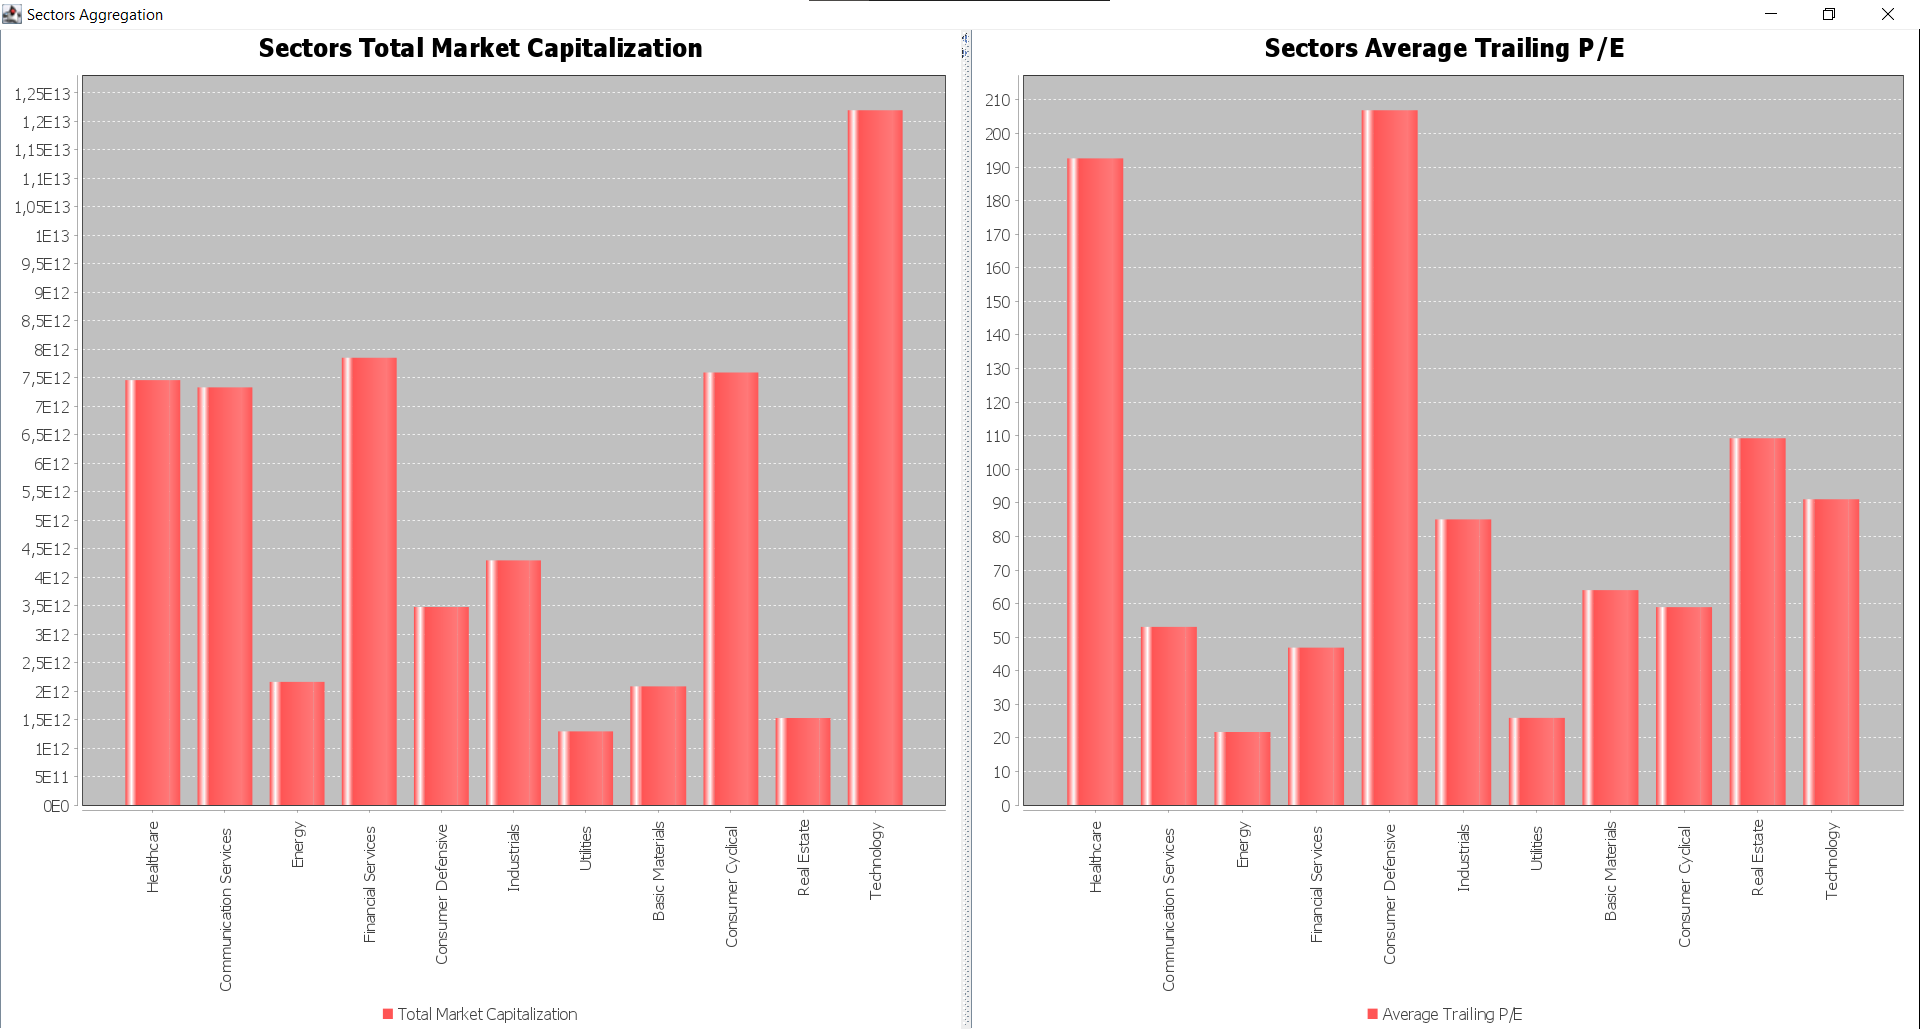
\includegraphics[scale=0.28]{img/user_manual/sector_aggregation.png}\\
}

\begin{lstlisting}[basicstyle=\footnotesize\ttfamily,language={},numbers=left,
numberstyle=\footnotesize,numbersep=8pt,frame=single]
> sector-search
Sector Name: Energy
[ BROG, PSXP, KOS, GMLP, CLMT, NCSM, PFIE, CCLP, NGS, WES, ENSV, FTSI, AXAS, EC, DEN, TTI, NBLX, E, GTE, PSX, PED, NNA, VVV, PVL, AR, HP, CEQP, MUR, DK, RTLR, LEU, NGL, NFG, PTEN, MMLP, PAGP, NESR, NR, PBFX, TRMD, BKR, NOG, ... ]
\end{lstlisting}

The search by country is similar to the search by sector: it also opens two bar charts with aggregated data by country and returns a list of the symbols of all the stocks belonging to the specified country.
\begin{lstlisting}[basicstyle=\footnotesize,language={},numbers=left,
numberstyle=\footnotesize,numbersep=8pt,frame=single]
> country-search
Country Name: Italy
[ E, NTZ, KLR, RACE, ]
\end{lstlisting}
\subsection{View stock}

The \texttt{view-stock} option allows the user to see the evolution of a stock in the market for a specific time range.\\
It asks the user for the stock symbol, the start and end dates and the day granularity, and then shows both a candlestick chart and a line chart of that stock for the desired time interval, along with printing all the information about that stock.

\begin{lstlisting}[basicstyle=\footnotesize\ttfamily,language={},numbers=left,
numberstyle=\footnotesize,numbersep=8pt,frame=single]
> view-stock
Ticker Symbol: TSLA
Start Date [YYYY-MM-DD]: 2021-01-01
End Date [YYYY-MM-DD]: 2021-01-10
Days granularity: 1
Short Name: Tesla, Inc.
Long Name: Tesla, Inc.
Symbol: TSLA
Quote type: EQUITY
Market capitalization: 8.00041992192E11
PE ratio: 1265.3346
Market: us_market
Exchange timezone short name: EST
Exchange timezone name: America/New_York
Sector: Consumer Cyclical
Industry: Auto Manufacturers
Currency: USD
Location:  3500 Deer Creek Road Palo Alto CA United States
650-681-5000
Logo URL: https://logo.clearbit.com/tesla.com
Website: http://www.tesla.com
Long business summary:
Tesla, Inc. designs, develops, manufactures, leases, and sells electric
vehicles, and energy [...]
\end{lstlisting}

\hfill \break
{\centering
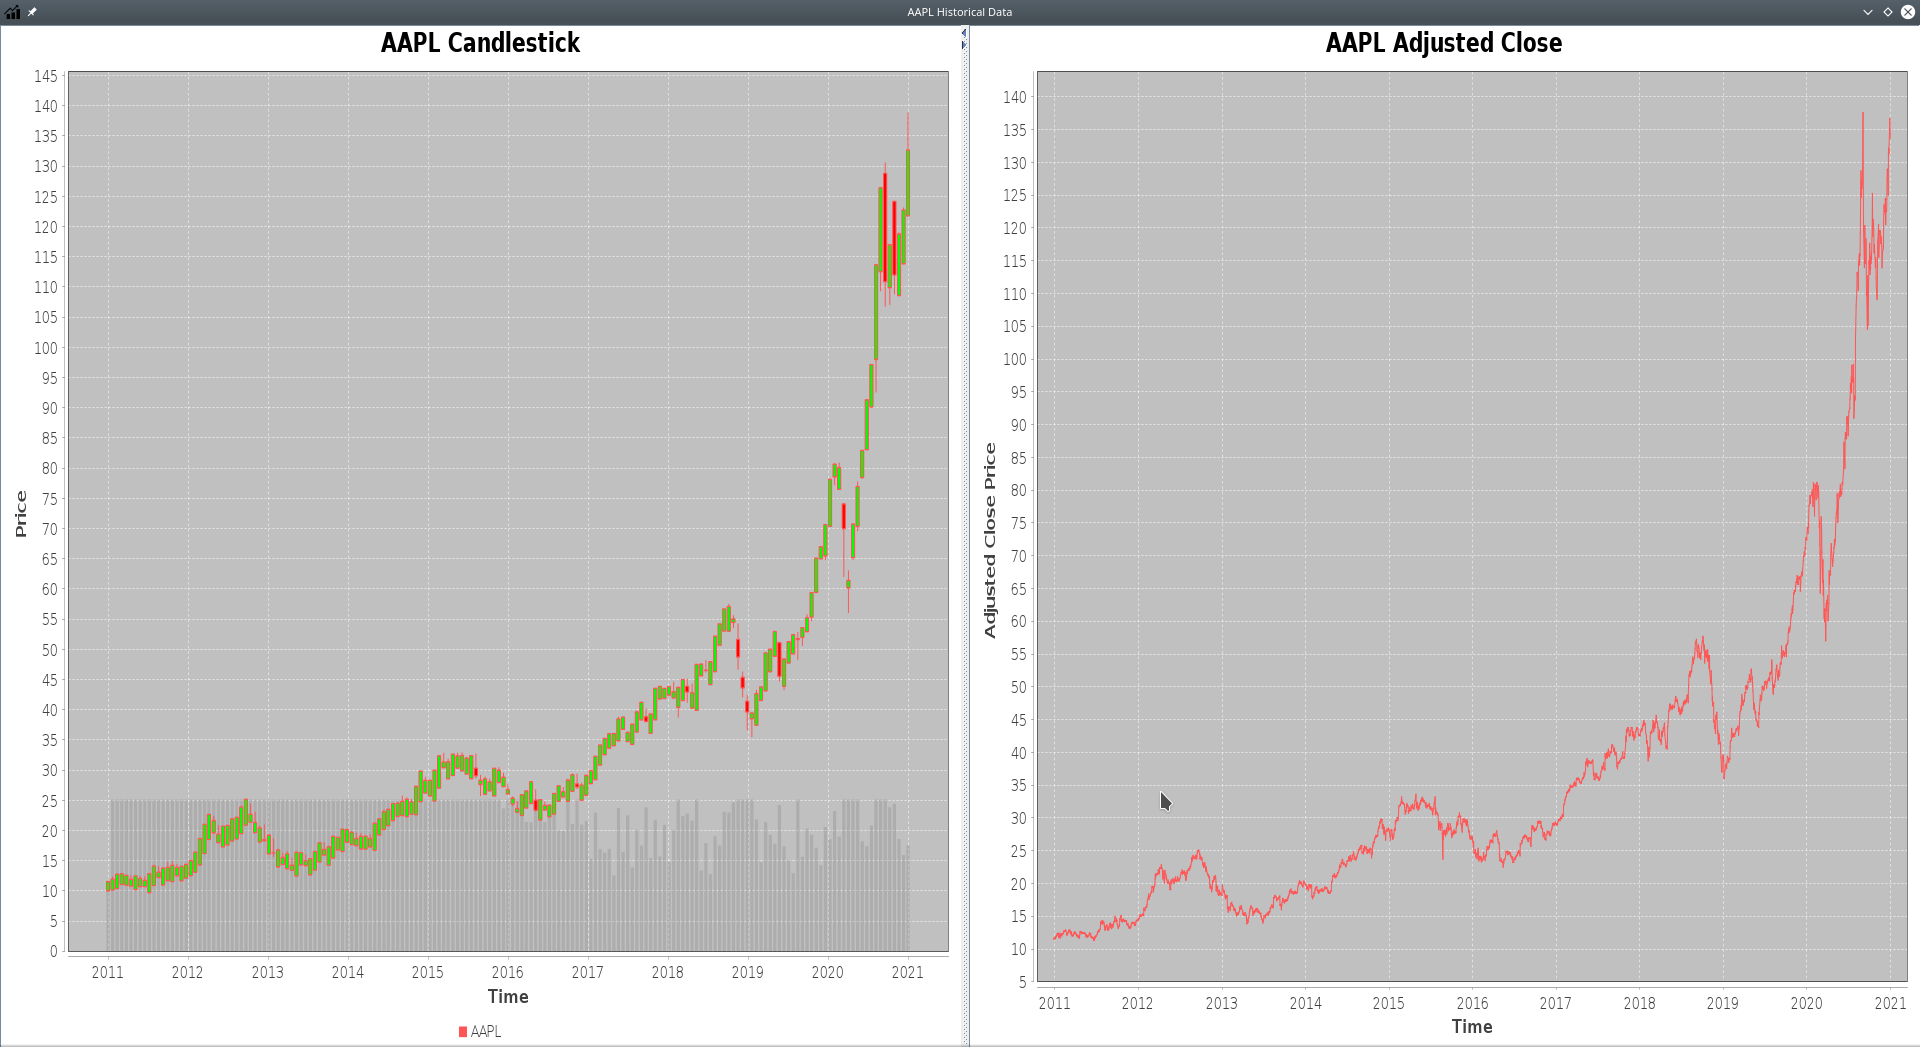
\includegraphics[scale=0.32]{img/user_manual/view_stock.png}\\
}

\subsection{Create portfolio}
The \texttt{create-portfolio} option allows the user create a new portfolio and insert stocks into it.\\
The user is first required to insert a name for the new portfolio and then to type a list of comma-separated symbols of the stocks they wish to insert in the portfolio.

\begin{lstlisting}[basicstyle=\footnotesize\ttfamily,language={},numbers=left,
numberstyle=\footnotesize,numbersep=8pt,frame=single]
> create-portfolio
Portfolio name: Portfolio1
Ticker Symbols [comma separated]: TSLA, MSFT, RACE
Portfolio created correctly.

\end{lstlisting}

\subsection{List portfolios}
The \texttt{list-portfolios} option shows the user a list of all their portfolios and the stocks each one of them is made of.\\

\begin{lstlisting}[basicstyle=\footnotesize\ttfamily,language={},numbers=left,
numberstyle=\footnotesize,numbersep=8pt,frame=single]
> list-portfolios
Portfolio1: [ TSLA, MSFT, RACE, ]
FAANG: [ FB, AAPL, AMZN, NFLX, GOOGL, ]
\end{lstlisting}

\subsection{View portfolio}
The \texttt{view-portfolio} option allows the user to view the composition of one of their portfolios. It prompts the user for the name of the portfolio to be viewed and then shows a pie chart of the portfolio.\\

{\centering
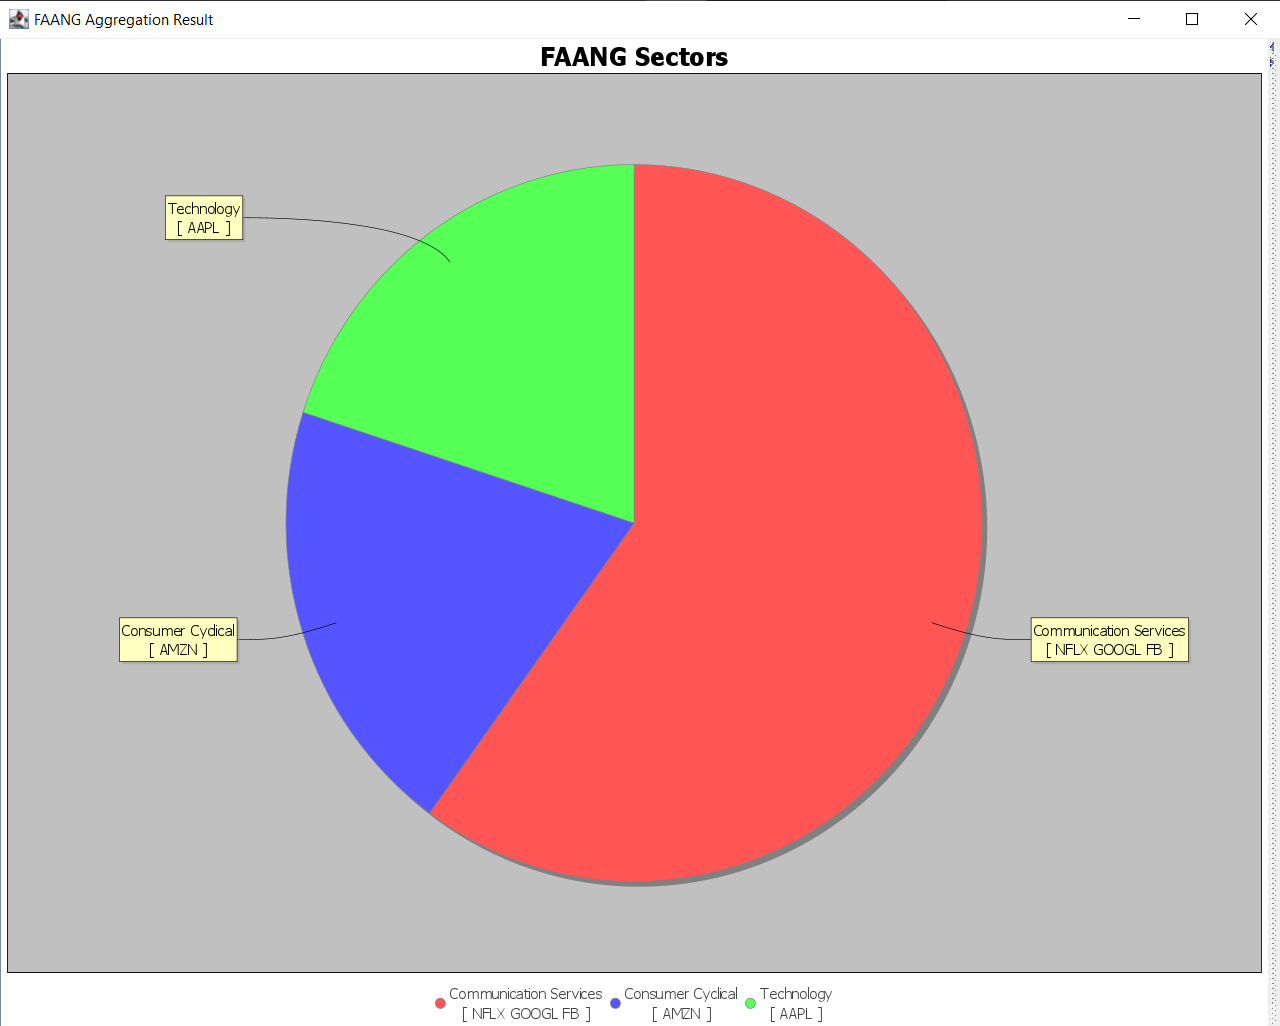
\includegraphics[scale=0.32]{img/user_manual/view_portfolio.png}\\
}

\subsection{Simulate portfolio}
TODO

\subsection{Delete portfolio}
The \texttt{delete-portfolio} option allows the user to delete one of their portfolios. It prompts the user for the name of the portfolio to be deleted and then it deletes the portfolio.

\section{StockSim Client Admin Mode}

After launching the application in \textit{admin} mode and logging in with admin credential, the following options are available:

\begin{lstlisting}[basicstyle=\footnotesize\ttfamily,language={},numbers=left,
numberstyle=\footnotesize,numbersep=8pt,frame=single]
> login
Username: admin
Password: stocksim
Admin login executed correctly.
Welcome StockSim Admin.
Available Commands:
add-ticker         add a new ticker symbol to the database.
add-admin          create new admin account.                                                                                                                                                                     
remove-admin       delete admin account.                                                                                                                                                                         
remove-user        delete user account.                                                                                                                                                                          
logout             logout from current admin account.                                                                                                                                                            
quit               quit StockSim client.  
\end{lstlisting}

\subsection{Add ticker}
The \texttt{add-ticker} option allows an admin to add a ticker to the database, provided it exists in the Yahoo! Finance database.
The underlying function retrieves the data from YFinance and loads it into the application database.

\begin{lstlisting}[basicstyle=\footnotesize\ttfamily,,language={},numbers=left,
numberstyle=\footnotesize,numbersep=8pt,frame=single]
> add-ticker
Ticker symbol: LSMSDB
Asset Profile created with success. Updating historical data.
Historical data updated with success.
\end{lstlisting}

\subsection{Add admin}
The \texttt{add-admin} option allows an admin to add other admin.
\begin{lstlisting}[basicstyle=\footnotesize\ttfamily,language={},numbers=left,
numberstyle=\footnotesize,numbersep=8pt,frame=single]
> add-admin
Admin account name: John
Admin account surname: Doe
Admin account username: admin2
Admin account password: stocksim
New admin account created.
\end{lstlisting}

\subsection{Remove admin}

The \texttt{remove-admin} option allows an admin to remove another admin from their role.

\begin{lstlisting}[basicstyle=\footnotesize\ttfamily,language={},numbers=left,
numberstyle=\footnotesize,numbersep=8pt,frame=single]
> remove-admin
Admin account username: admin2
Admin account password: stocksim
Admin account deleted.
\end{lstlisting}

\subsection{Remove user}
The \texttt{remove-user} option allows an admin to delete a user from the database.

\begin{lstlisting}[basicstyle=\footnotesize\ttfamily,language={},numbers=left,
numberstyle=\footnotesize,numbersep=8pt,frame=single]
> remove-user
User account email: jsmith@example.com
User account deleted.
\end{lstlisting}

